\documentclass{article}
\usepackage{amsmath}
\usepackage{amssymb}
\usepackage{amsthm}
\usepackage{accents}
\usepackage[utf8]{inputenc}
\usepackage{enumitem}
\setlength{\parskip}{1em}
\usepackage{titlesec}
\usepackage{tikz}

\titleformat{\section}[hang]{\sc\Large}{\S\thesection}{3ex}{}[]
\titleformat{\subsection}[hang]{\sc\large}{\S\thesubsection}{3ex}{}[]
\titleformat{\subsubsection}[hang]{}{\S\thesubsubsection}{3ex}{}[]
\setcounter{section}{-1}
\newcommand{\coord}{co{\"o}rdinate }
\newcommand{\coords}{co{\"o}rdinates }
\newcommand{\bhat}[1]{\boldsymbol{\hat{#1}}}

\newcommand{\ihat}{\ {\hat{\textbf{i}}}}
\newcommand{\jhat}{\ {\hat{\textbf{j}}}}
\newcommand{\khat}{\ {\hat{\textbf{k}}}}
\newcommand{\rhat}{\ {\hat{\textbf{r}}}}
\newcommand{\that}{\ \boldsymbol{\hat{\theta}}}

\renewcommand{\d}{\text{d}}
\renewcommand{\vec}[1]{\accentset{\rightharpoonup}{\text{#1}}}

\newcommand{\vecdot}[2]{\vec{#1}\cdot\d \vec{#2}}

\theoremstyle{definition}
\newtheorem{example}{Example}[section]

\title{Vector Calculus}
\date{}

\begin{document}

\maketitle

\section{Co{\"o}rdinate Systems}

\subsection{Converting }

\subsubsection{Polar \coords}

A point $P$ in Cartesian \coords $(x, y)$ has polar \coords $(r, \theta)$  

\begin{alignat*}{2}
    r &= (x^2 + y^2)^{\frac{1}{2}} \qquad\qquad &x = r\cos \theta\\
    \theta &= \arctan\left(\frac{1}{2}\right) \qquad\qquad &y = r\sin \theta
\end{alignat*}

The unit vectors in polar \coords are converted to and from as such

\begin{alignat*}{2}
    \rhat&= \cos\theta\ihat + \sin\theta\jhat \qquad\qquad &\ihat = \cos\theta\rhat - \sin\theta\that\\
    \that &= -\sin\theta\ihat + \cos\theta\jhat \qquad\qquad &\jhat = \sin\theta\rhat + \cos\theta\that
\end{alignat*}

The same applies to their components, for some arbitrary vector $\vec{v}$

\begin{alignat*}{2}
    v_r &= v_x\cos\theta + v_y\sin\theta \qquad\qquad &v_x = v_r\cos\theta - v_\theta\sin\theta\\
    v_\theta &= -v_x\sin\theta + v_y\cos\theta \qquad\qquad &v_y = v_r\sin\theta + v_\theta\cos\theta
\end{alignat*}

\section{Integral Vector Calculus}

\subsection{Line integrals}

A line of path integral is the integral of a scalar or vector field along a specified path $C$ from point $A$
to point $B$, there are three general forms.
$$\vec{I} = \int_C \text{F} \d\vec{l} \qquad\quad \vec{I} = \int_C \vec{F}\cdot \d\vec{l} \qquad\quad \vec{I} = \int_C \vec{F}\times \d\vec{l}$$
Where d$\vec{l}$ is the infitesimal line element, remember that it is different for each \coord system.
The direction of the path matters, if the path is reversed, as in from $B$ to $A$, then d$\vec{l}$ becomes $-$d$\vec{l}$

If $A$ and $B$ are the same point then the integral is \emph{closed}, and as such is written $\oint$. By convention
the path taken for a closed integral is anti-clockwise (widdershins).

\begin{example}
    Calculate the line integral $\int_C \vec{A}\cdot \d\vec{l}$ where $\vec{A} = (x + y)\ihat\ +\ (y-x)\jhat$ along the path
    $y = x^2$ from $(1, 1)$ to $(2, 4)$

    The first step is to evaluate the dot product inside the integral. It is clear we should be using Cartesian 
    \coords and so $\d\vec{l} = \d x\ihat + \d x\jhat + \d z\khat$
    $$\vec{A}\cdot\d\vec{l} = (x + y)\d x + (y - x)\d y$$
    $x$ and $y$ are not independent along the path, i.e. a change in x produces a change in y.
    Whilst not always possible, it is much easier if we contract our integral down to one variable.
    \begin{align*}
        y &= x^2\\
        \frac{dy}{dx} &= 2x\\
        \vec{A}\cdot\d\vec{l} &= (x+x^2)\ \d x + (x^2-x)2x\ \d x\\
        \vec{A}\cdot\d\vec{l} &= 2x^3 - x^2 + x\ \d x\\
        \int_C \vec{A}\cdot \d\vec{l} &= \int_C 2x^3 - x^2 + x\ \d x
    \end{align*}
    Now we need to determine our limits, we are integrating with respect to $x$, and our path is from $(1, 1)$ to $(2, 4)$
    to our limits are from 1 to 2. The order is very important so make sure to double check.
    \begin{align*}
        \int_1^2 2x^3 - x^2 + x\ \d x &= \left[\frac{2x^4}{4}-\frac{x^3}{3}+\frac{x^2}{2}\right]_1^2\\
        &= \frac{22}{3} - \frac{2}{3} = \frac{20}{3}
    \end{align*}
\end{example}

\begin{example}
    Calculate the line integral $\oint_C \vec{F}\cdot \d\vec{l}$ where $\vec{F} = x^2y\ihat + 3xy\jhat$ around 
    a unit square with vertices at $(0,0),\ (1,0),\ (1,1),\ (0,1)$.
    \begin{center}
        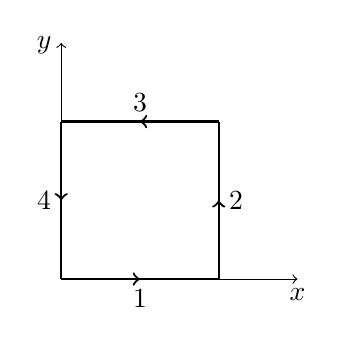
\begin{tikzpicture}[x=2cm, y=2cm]
            \draw[->] (0,0) -- (0,1.5) node[anchor=mid east]{$y$};
            \draw[->] (0,0) -- (1.5,0) node[anchor=north]{$x$};
            \draw[thick] (0,0) -- (1,0) node[anchor=north,midway]{$1$};
            \draw[thick,->] (0,0) -- (0.5,0);
            \draw[thick] (1,0) -- (1,1) node[anchor=west,midway]{$2$};
            \draw[thick,->] (1,0) -- (1,0.5);
            \draw[thick] (1,1) -- (0,1) node[anchor=south,midway]{$3$};
            \draw[thick,->] (1,1) -- (0.5,1);
            \draw[thick] (0,1) -- (0,0) node[anchor=east,midway]{$4$};
            \draw[thick,->] (0,1) -- (0,0.5);
        \end{tikzpicture}
    \end{center}


    For this problem we need to break it down into pieces, namely each side. It does not matter which order 
    we evaluate our sides, only that we evaluate them anti-clockwise, i.e. from (0,0) to (0,1).

    Side 1: (0,0) to (0,1),\ $y = 0,\ x: 0 \rightarrow 1,\ \vec{F} = 0\ihat + 0\jhat$ so $\int \vecdot{F}{l} = 0$

    Side 2: (0,1) to (1,1),\ $x = 0,\ y: 0\rightarrow 1,\ \vec{F} = y\ihat + 3y\jhat$ \\
    Now we need to find d$\vec{l}$, since $\vec{F}$ only points in the $\jhat$ direction on this side we can say d$\vec{l}$ = d$y\jhat$.
    \begin{align*}
        \vecdot{F}{l} &= 3y\ \d y\\
        \int_0^1 \vecdot{F}{l} &= \int_0^1 3y\ \d y \\
        &= \left[\frac{3y^2}{2}\right]_0^1 = \frac{3}{2}
    \end{align*}

    Side 3: (1,1) to (0,1),\ $y = 0,\ x: 1\rightarrow 0,\ \vec{F} = x^2\ihat + 3x\jhat$\\
    d$\vec{l}$ only moves in the x direction so d$\vec{l}$ = d$x\ihat$.
    \begin{align*}
        \vecdot{F}{l} &= x^2\d x\\
        \int_1^0 x^2 \d x &= \left[\frac{x^3}{3}\right]_1^0 = \frac{-1}{3}
    \end{align*}
    Ensure the limits are in the right order!!

    Side 4: (0,1) to (0,0),\ $x = 0,\  y: 1\rightarrow 0,\ \vec{F} = 0\ihat + 0\jhat$ so $\int \vecdot{F}{l} = 0$

    So $\oint\vecdot{F}{l} = \frac{3}{2} - \frac{1}{3} = \frac{7}{6}$
\end{example}

\end{document}
